\documentclass{article}
\usepackage[margin=1in]{geometry}
\usepackage{booktabs}
\usepackage{graphicx}
\title{Reporte de carga MQTT}
\author{Autogenerado por mqtt\_stress\_async.py}
\date{}
\begin{document}
\maketitle
\section*{Resumen de la corrida}
\begin{tabular}{ll}\topruleSesión & async-run-20251205-203826-s00000-n00400 \ CSV & ..\textbackslash\{\}async-run-20251205-203826-s00000-n00400-metrics.csv \ Dispositivos & 400.000 \ Publicaciones OK & 1.43e+05 \ Publicaciones fallidas & 0.000 \ Latencia promedio (ms) & 19.620 \ Latencia P95 (ms) & 44.335 \ Mensajes por segundo & 79.656 \ Ancho de banda (Mbps) & 0.101 \ Volumen de datos (MB) & 21.665 \ Duración (s) & 1.8e+03 \ \bottomrule\end{tabular}
\subsection*{Gráficos}
\begin{figure}[h]
\centering
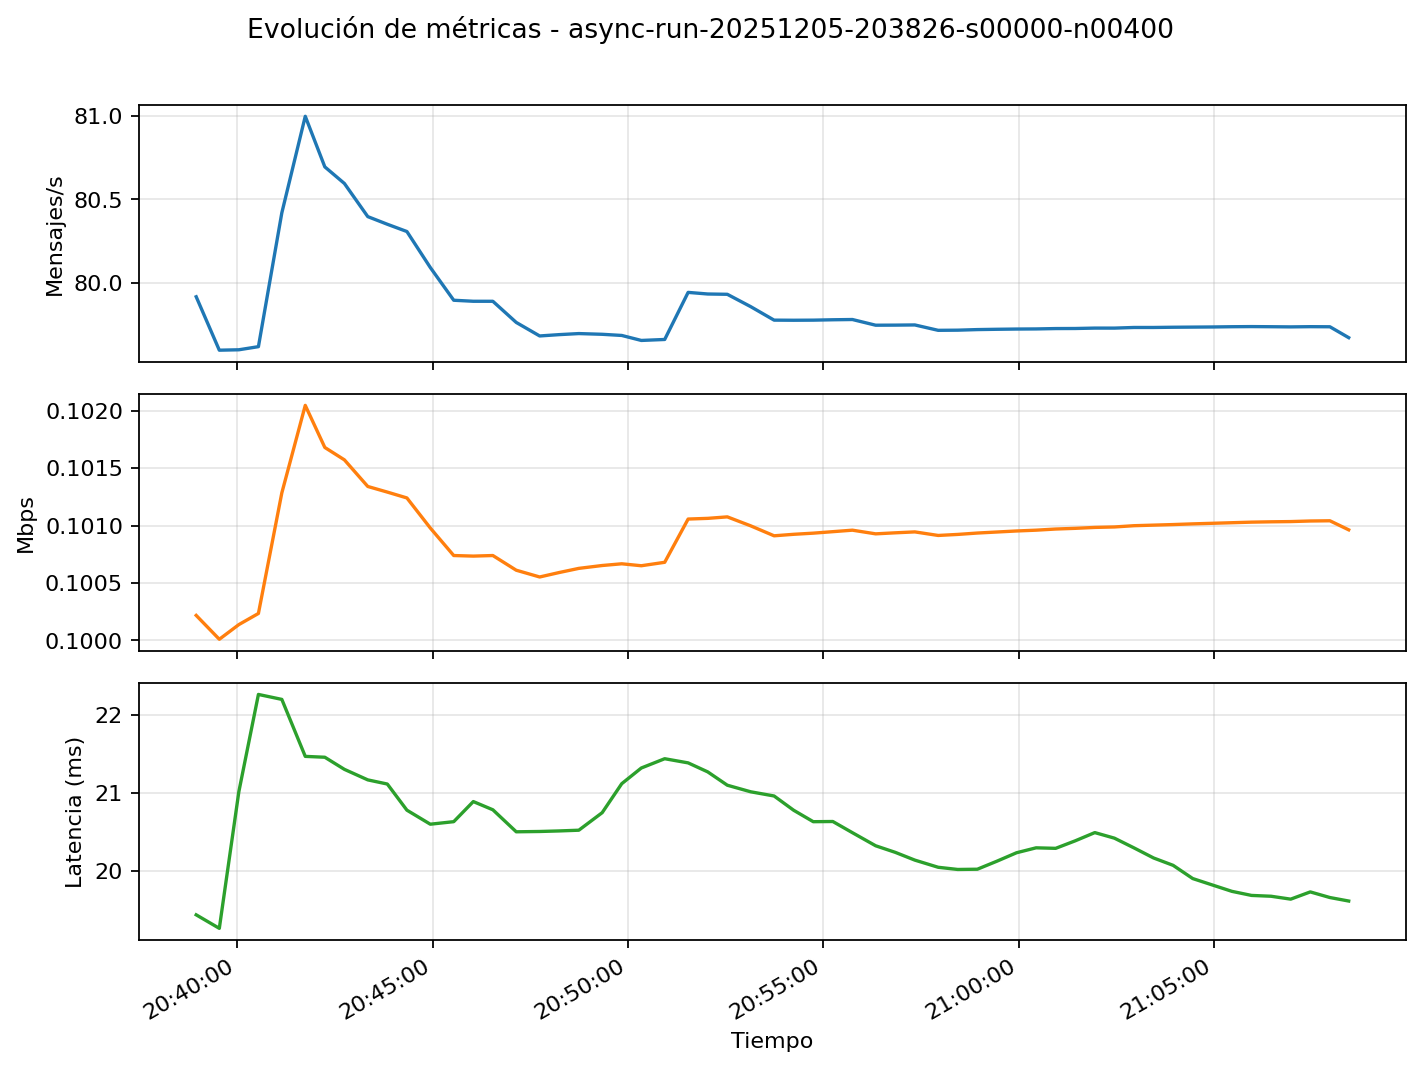
\includegraphics[width=0.9\linewidth]{async-run-20251205-203826-s00000-n00400-overview.png}
\caption{Mensajes/s, ancho de banda y latencia promedio.}
\end{figure}

\subsection*{Fuente de datos}
El CSV original se encuentra en \texttt{..\textbackslash\{\}async-run-20251205-203826-s00000-n00400-metrics.csv}.\\
Este documento se genera automáticamente tras cada corrida.\
\end{document}
